\documentclass[a4paper,12pt]{article}

\usepackage[russian]{babel}
\usepackage{cmap}
\usepackage[utf8]{inputenc}
\usepackage[usenames]{color}
\usepackage{tabularray}
\usepackage{xcolor}
\usepackage{graphicx} 
\usepackage{subfigure}
\usepackage{subcaption}

\usepackage[unicode]{hyperref} % цвета гиперссылок
\hypersetup{
	colorlinks,
	citecolor=black,
	filecolor=black,
	linkcolor=blue,
	urlcolor=black
}

\usepackage{geometry} % задаёт поля 
%\geometry{left=3cm}
%\geometry{right= 1.5cm}
%\geometry{top=2cm}
%\geometry{bottom=2cm} 

\usepackage{enumitem} % настраивает работу со списками:
\def\labelitemi{—} % ... задаёт длинное тире как стандартный маркер ненумерованного списка
\setlist{nolistsep} %  ... убирает дополнительный отступы между элементами списка


% удаляет названия и продолжение следует и т. для таблиц, будет только таблица без всего
\DefTblrTemplate{contfoot-text}{default}{}
\DefTblrTemplate{conthead-text}{default}{}
\DefTblrTemplate{caption}{default}{}
\DefTblrTemplate{conthead}{default}{}
\DefTblrTemplate{capcont}{default}{}


\title{Настройка параметров кластеризации DBSCAN по значениям метрики силуэта }
\author{В. Г. Мосин}
\date{}

%   \input{preamble.tex}
\begin{document}
	\maketitle
	\abstract{\noindent  В настоящей статье рассматривается метод автоматической настройки параметров кластеризации DBSCAN, основанный на авторском алгоритме определения локтевой точки метрики силуэта. Излагается алгоритм настройки и его приложения к наборам синтетических данных.}
	
\tableofcontents
	
\section{Введение}
Кластеризация является одним из основных методов анализа данных, который позволяет разделить множество объектов на группы, называемые кластерами, таким образом, чтобы объекты внутри одного кластера были более похожи друг на друга, чем на объекты из других кластеров. Этот подход играет важную роль в различных областях, таких как машинное обучение, статистика и многих других (см. [4]).

Верный подбор параметров кластеризации является критически важным этапом процесса анализа данных. Параметры кластеризации определяют, какие именно свойства объектов будут учитываться при формировании кластеров. Неправильный выбор параметров может привести к некорректному образованию кластеров, а значит, к неверной интерпретации данных и неправильным выводам.


\subsection{Теоретическая часть}

В нашей работе мы проанализируем один из методов автоматической настройки параметров кластеризации DBSCAN, используя в качестве метрики ее эффективности метрику силуэта.

\subsubsection{Кластеризация DBSCAN}

Кластеризация DBSCAN (Density-Based Spatial Clustering of Applications with Noise) — это алгоритм машинного обучения, который используется для группировки данных на основе их плотности. В отличие от других методов кластеризации, таких как KMeans или агломеративная кластеризация, алгоритм DBSCAN способен обнаруживать кластеры произвольной и сложной формы, а также находить шумовые точки, которые не принадлежат ни одному кластеру. DBSCAN является мощным инструментом для кластеризации данных и находит применение в различных областях, таких как анализ социальных сетей, геоинформационные системы, анализ изображений и т. д. Его способность обнаруживать кластеры произвольной формы и игнорировать шумовые данные делает его очень полезным инструментом для извлечения информации из больших объемов данных.

\subsubsection{Метрика силуэта}

Метрика силуэта является одной из ключевых метрик, которая используется для оценки качества кластеризации. Она позволяет измерить, насколько хорошо объекты распределены по кластерам, и определить, насколько каждый объект подходит своему кластеру. Принцип работы метрики силуэта основывается на оценке плотности и компактности кластеров. На высокий показатель силуэта влияют два фактора: среднее расстояние между объектом и остальными объектами в его кластере (компактность), а также среднее расстояние до объектов, принадлежащих другим кластерам (разделенность). Чем больше величина силуэта, тем лучше кластеризация.

Одним из основных преимуществ метрики силуэта является ее универсальность. В отличие от других метрик, она может быть применена к различным типам данных и алгоритмам кластеризации. Эта метрика не требует априорного знания количества кластеров, что является ее значительным преимуществом, а в применении к кластеризации DBSCAN, для которой число кластеров заранее неизвестно, метрика силуэта является незаменимой.

\subsection{Постановки задачи}
Когда исследователь применяет метод локтя, его действия состоят в визуальной оценке графика изучаемой метрики. За этими красивыми словами кроется тот факт, что исследователь определяют локтевую точку на глаз. И хотя при этом используются более корректные слова — визуально или интуитивно, сути это не меняет.

\subsubsection{Предмет исследования}

 Ключевым фрагментом нашего алгоритма настройки параметров кластеризации DBSCAN является функция автоматического определения локтевой точки (см. п. 2). Мы будем исследовать работу этой функции.

\subsubsection{Методика исследования} 

Мы реализуем алгоритм настройки и протестируем его на достаточном количестве синтетических данных.

\subsubsection{Цель исследования} 

Наша цель — выяснить, является ли предложенный нами метод автоматической настройки параметров кластеризации DBSCAN самостоятельным рабочим инструментом, не требующим вмешательства человека, и, по возможности, установить границы применения этого метода.

\subsection{Библиотеки}
Для выполнения вычислений и анализа данных мы пользуемся средой \texttt{Jupyter Notebook}, которая предоставляет удобные средства для работы с языком программирования Python и его главными библиотеками: \texttt{NumPy}, \texttt{Pandas}, \texttt{sklearn} и \texttt{matplotlib}. Благодаря этим инструментам, мы можем эффективно работать с данными, выполнять исследования и визуализировать результаты (см. [1], [2]). 

%Библиотека \texttt{numpy} является одной из ключевых библиотек для научных вычислений и обработки массивов данных в языке программирования \texttt{Python}. Библиотека \texttt{pandas}~--- одна из наиболее популярных и мощных библиотек для работы с данными в языке программирования \texttt{Python} (см. [1]). 
%
%Библиотека \texttt{scikit-learn}, широко известная как \texttt{sklearn}, предоставляет обширный набор инструментов и функций для решения различных задач в языке программирования Python, таких как задачи классификации, регрессии, кластеризации и др. Мы используем эту библиотеку для решения регрессионных задач.


\section{Функция \textbf{\texttt{fold\_point}}}

В теле алгоритма (см. п. 3) мы осуществим прогон кластеризации DBCSAN по двумерной сетке ее двух основных параметров:

\medskip\noindent 
\begin{enumerate}
	\item \texttt{eps} — радиус, внутри которого точки облака данных учитываются, как принадлежащие одному кластеру;
	\item \texttt{min\_samples} — число точек, начиная с которого фрагмент облака может считаться самостоятельным кластером.
\end{enumerate}

\medskip\noindent 
При этом для оценки качества кластеризации мы будем использовать метрику силуэта \texttt{silhouette\_score}, которая принимает значения из промежутка [–1, 1], и качество кластеризации оценивается тем выше, чем больше значение \texttt{silhouette\_score}-метрики.

Однако при таком вполне очевидном подходе возникает одна из существенных проблем подбора параметров кластеризации DBCSAN. Она состоит в том, что лучшая кластеризация далеко не всегда соответствует лучшему значению метрики. 


\begin{figure}[!h]
	\centering
	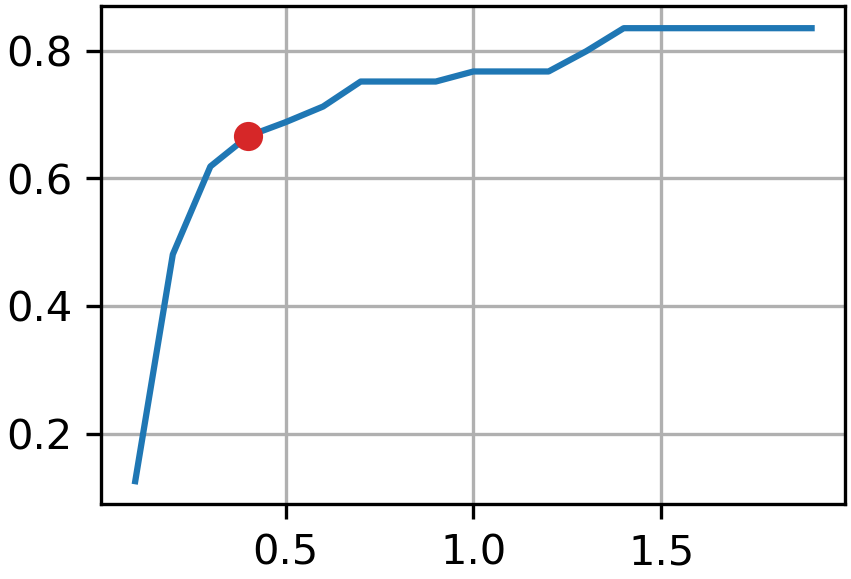
\includegraphics[width=0.4\linewidth]{pictures/Локтевая метрика}
	\hspace{0.05\linewidth}
	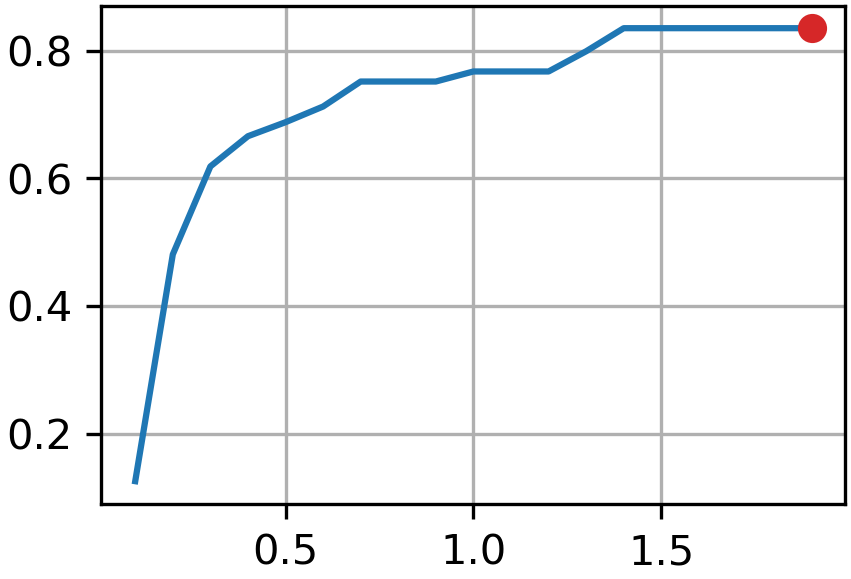
\includegraphics[width=0.4\linewidth]{pictures/Максимальная метрика}\\
	\caption{Локтевое значение метрики и ее максимальное значение}
\end{figure}


Максимальное значение метрики силуэта (см. р. 1(b)) может привести к тому, что все объекты будут объединены в один кластер (плюс, возможно, некоторое количество выбросов), а это не самая лучшая кластеризация, так как она вообще не улавливает каких-либо различий между объектами. При этом разумное разделение на кластеры происходит при так называемом локтевом значении метрики (см. р. 1(a)), которое не определяется математически. Это не точка экстремума и не точка перегиба (хотя иногда в литературе ее называют именно так, что является грубейшей ошибкой), это не точка максимальной кривизны и т. д. Локтевое значение метрики требует интуиции и опыта исследователя.

Обычно говорят, что локтевая точка — это точка, после прохождения которой уже не происходит существенного изменения метрики. Не претендуя на строгое определение локтевой точки (которое, видимо, невозможно), мы предлагаем собственный метод ее нахождения. Мы хотим избавиться от человеческого фактора в процессе локализации локтевой точки и исключить те самые «интуицию и опыт исследователя», а наоборот: дать формальный автоматический алгоритм, возвращающий локтевую точку.

Наша идея состоит в том, чтобы осуществить ансаблирование одномерной линейной регрессионной модели путем разбиения промежутка изменения предиктора метрики силуэта на два интервала (см. [5], [6]). Напомним, что оценка линейной регрессионной модели проводится при помощи коэффициента детерминации $R^2 = 1 - S^*/S’$, где:


\medskip\noindent
\begin{enumerate}
	\item $S^*$ — сумма квадратов отклонений прогнозируемых значений целевой функции от ее истинных значений,
	\item $S’$ — сумма квадратов отклонений истинных значений целевой функции от ее среднего значения.
\end{enumerate}

\medskip\noindent
Если разбить промежуток изменения предиктора на два участка, построить на каждом из них линейную модель и вычислить совокупный коэффициент детерминации для ансамбля из двух моделей, то суммарное отклонение в знаменателе останется точно таким же, но суммарное отклонение в числителе станет меньше (см. рис. 2).

\begin{figure}[!h]
	\centering
	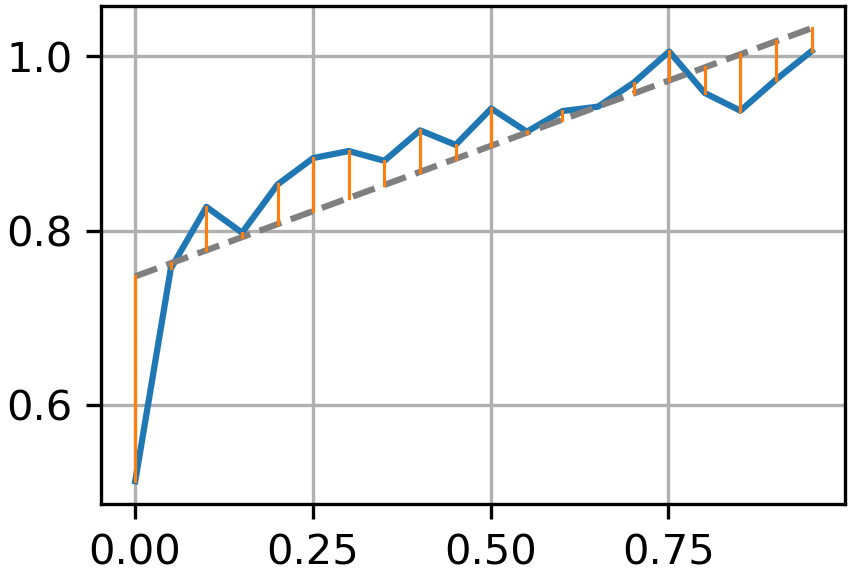
\includegraphics[width=0.4\linewidth]{pictures/Без ансамбля}
	\hspace{0.05\linewidth}
	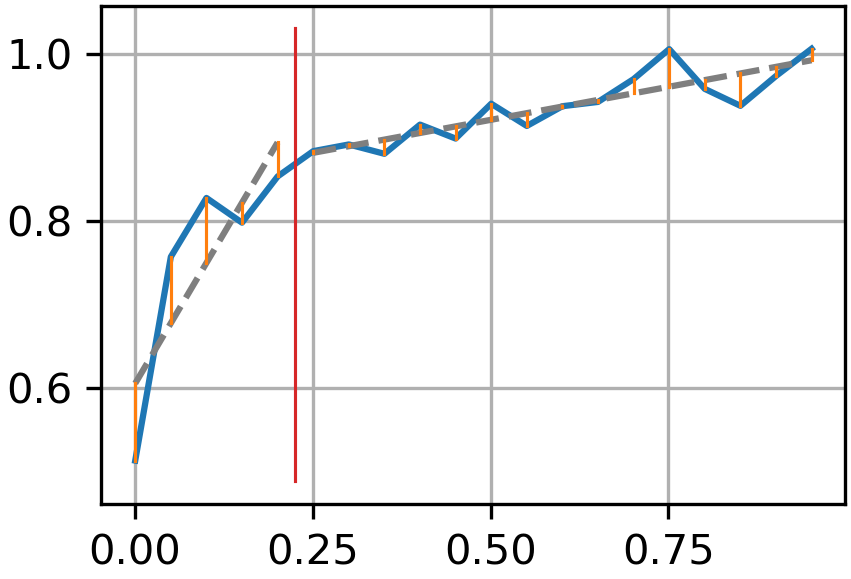
\includegraphics[width=0.4\linewidth]{pictures/С ансамблем}\\
	\caption{Линейная модель (a) и ансамбль из двух линейных моделей (b)}
\end{figure}

Это приводит к повышению коэффициента детерминации (см. [6]). 

Теперь, если выполнить цикл по одномерной сетке, разбивающей промежуток изменения предиктора, получим список коэффициентов детерминации возникающих при этом ансамблей, среди которых окажется какой-то максимальный элемент. Индекс этого элемента списка мы и примем в качестве абсциссы локтевой точки (еще раз повторим, что это не определение локтевой точки, а рабочий метод ее нахождения).

Подробное описание алгоритма функции, определяющей локтевую точку, выходит за рамки настоящей статьи, которая посвящена не локтевым точкам, а кластеризации DBSCAN, поэтому мы ограничимся лишь указанием ее основных характеристик: 

\medskip\noindent
\begin{enumerate}
	\item имя функции  — \texttt{fold\_point};
	\item аргументы функции — пара одномерных массивов \texttt{A}, \texttt{B}, обладающих равной длиной, причем, первый массив содержит значения горизонтальной переменной, а второй — вертикальной;
	\item в теле функции реализован алгоритм, основанный на изложенной выше идее ансаблирования линейной регрессионной модели для метрики силуэта;
	\item функция возвращает номер элемента массива \texttt{A}, в котором фиксируется локтевое значение массива \texttt{B}.
\end{enumerate}

\section{Алгоритм}

\subsection{Генерация синтетических данных}
Для реализации нашего алгоритма настройки кластеризации DBCSAN мы используем синтетические данные. Мы импортируем специальный модуль \texttt{datasets} библиотеки \texttt{sklearn}, после чего нам становится доступен метод  \texttt{make\_blobs}, при помощи которого мы генерируем двумерные данные. На старте алгоритма мы создаем облако из 500 точек и записываем его в двумерный массив \texttt{X}.

\subsection{Двумерная сетка метрики силуэта}

Сетка для вложенного цикла должна учитывать специфику параметров \texttt{eps} и \texttt{min\_samples}. Параметр \texttt{eps} задает радиус, внутри которого рассчитывается плотность облака, то есть по своей природе это непрерывный параметр, мы будем варьировать его в пределах от 0.1 (так как нулевой радиус не имеет смысла) до 2 с шагом 0.1. Для задания сетки по параметру \texttt{eps} мы применяем метод \texttt{arange} библиотеки \texttt{numpy}:

\medskip\noindent
\texttt{eps\_grid = np.arange(0.1, 2, 0.1)}

\medskip\noindent
Второй параметр \texttt{min\_samples} задает количество объектов, то есть по своей природе является натуральным числом, и мы варьируем его в пределах от 1 (но не от 0) до 15 с шагом 1. Для задания сетки по параметру \texttt{min\_samples} мы также применяем метод \texttt{arange} библиотеки \texttt{numpy}:

\medskip\noindent
\texttt{min\_samples\_grid = np.arange(1, 15, 1)}


\subsection{Таблица метрик}


Мы будем обучать модель кластеризации DBCSAN для каждой пары значений параметров \texttt{eps} и \texttt{min\_samples} и вычислять соответствующую этим значениям величину метрики \texttt{silhouette\_score}. Таким образом, все возможные значения метрики силуэта, которые возникнут по результатам вложенного цикла по сетке, естественным образом заполнят таблицу с двумя входами: столбцы таблицы будут нумероваться значениями \texttt{eps}, а строки — значениями \texttt{min\_samples}.

В начале работы алгоритма, еще до исполнения цикла по сетке мы вызываем метод \texttt{DataFrame} библиотеки \texttt{pandas}, передаем ему в качестве значения параметра columns значение переменной \texttt{eps\_grid}, а в качестве значения параметра \texttt{index} — значение переменной \texttt{min\_samples\_grid}. Результат записываем в переменную \texttt{result}:

\medskip\noindent
\texttt{result = pd.DataFrame(columns=eps\_grid, index=min\_samples\_grid)}

\medskip\noindent
Таким образом, в начале алгоритма мы имеем датафрейм \texttt{result}, который полностью заполнен значениями \texttt{NaN}. Далее, для сокращения кода, а также для того, чтобы подчеркнуть табличную природу элементов сетки, вводим две переменные:

\medskip\noindent
\texttt{cols = result.columns\\
ind = result.index}


\medskip\noindent
Это два массива, по элементам которых и будет осуществляться вложенный цикл.


\subsection{Вложенный цикл по параметрам \texttt{eps} и\\ \texttt{min\_samples}}


\subsubsection{Стартовая итерация}

Присваиваем параметрам \texttt{eps} и \texttt{min\_samples} стартовые значения массивов \texttt{cols} и \texttt{ind} и, при помощи метода \texttt{DBCSAN} из модуля \texttt{clusters} библиотеки \texttt{sklearn} получаем модель кластеризации \texttt{clust}:


\medskip\noindent
\texttt{clust = DBSCAN(eps=cols[0], min\_samples=ind[0])}

\medskip\noindent
Обучаем модель на массиве \texttt{X} при помощи метода \texttt{fit} и выводим метки кластеров в список \texttt{labels} при помощи метода \texttt{labels\_}:

\medskip\noindent
\texttt{clust.fit(X)\\
labels = clust.labels\_}

\medskip\noindent
Далее нам нужно учесть ограничения метрики силуэта. Дело в том, что ее невозможно вычислить, если по результатам кластеризации с данными значениями параметров возникли следующие ситуации:

\medskip\noindent
\begin{enumerate}
	\item все объекты оказались объединены в единственный кластер (в этом случае отсутствует межкластерное различие),
	\item каждый объект оказался выделен в самостоятельный кластер (в этом случае отсутствует внутрикластерное сходство).
\end{enumerate}


\medskip\noindent
Поэтому для бесперебойной работы цикла при заполнении таблицы \texttt{result} должно выполняться условие: число получившихся кластеров больше 1 и меньше числа объектов в массиве \texttt{X}. Так как число кластеров — это число уникальных элементов в списке \texttt{labels}, мы применяем условный оператор \texttt{if} к следующему логическому выражению:

\medskip\noindent
\texttt{if (len(set(labels)) > 1) and (len(set(labels)) < len(X))}

\medskip\noindent
Если это условие выполняется, то в датафрейм \texttt{result} на место, расположенное в столбце с именем \texttt{cols[0]} и строке с индексом \texttt{ind[0]} записываем метрику силуэта, вычисленную при данных значениях параметров \texttt{eps} и \texttt{min\_smples}. Для этого применяем метод \texttt{silhouette\_score} из модуля \texttt{metrics} библиотеки sklearn к паре \texttt{(X, labels)} и выполняем присваивание:

\medskip\noindent
\texttt{result[cols[0]][ind[0]] = silhouette\_score(X, labels)}

\medskip\noindent
Напомним, что изначально датафрейм \texttt{result} заполнен значениями \texttt{NaN}. Поэтому, если условие присваивания не выполняется, то на соответствующей позиции остается \texttt{NaN}, если же оно выполняется, позиция заполняется значением метрики силуэта.

\subsubsection{Внутренний цикл по \texttt{min\_samples}}

Переходим к следующему значению массива \texttt{ind} и повторяем действия до исчерпания всех элементов массива. В результате в датафрейме \texttt{result} получаем заполненный первый столбец (за исключением тех позиций, для которых условие вычисления метрики силуэта оказалось невыполненным).

\subsubsection{Внешний цикл по eps}

Переходим к следующему значению массива \texttt{cols} и повторяем действия до исчерпания всех элементов массива. В результате получаем заполненный датафрейм \texttt{result} (за исключением тех позиций, для которых условие вычисления метрики силуэта оказалось невыполненным).


\subsection{Редукция таблицы результатов}


Итак, на этом шаге мы имеет таблицу \texttt{result}, заполненную метриками силуэта, вычисленными для различных значений параметров \texttt{eps} и \texttt{min\_samples}. Но некоторые позиции этой таблицы могут быть не заполнены в силу указанных выше причин. Мы удаляем из таблицы \texttt{result} все столбцы, в которых встречается хотя бы одно значение \texttt{NaN}. Для этого мы транспонируем датафрейм \texttt{result}, применяем метод \texttt{dropna} из библиотеки pandas и снова транспонируем то, что получилось:

\medskip\noindent
\texttt{result = result.T.dropna().T}

\medskip\noindent
Теперь в таблице \texttt{result} заполнены все поля, хотя количество столбцов в ней, скорее всего, уменьшилось.


\subsection{Лучшая строка в таблице результатов}


Визуально строки таблицы \texttt{result} представляют собой семейство кривых, где по горизонтали откладывается параметр \texttt{eps} (при фиксированном значении параметра \texttt{min\_smples}), а по вертикали — значение метрики силуэта (см. рис. 3(a)).

Если усреднить значения каждой такой кривой по всем возможным значениям горизонтальной переменной, то получится семейство горизонтальных линий, среди которых какая-то одна линия окажется самой верхней. Это будет означать, что соответствующая кривая по совокупности всех возможных значений горизонтальной переменной демонстрирует наилучший результат (см. рис. 3(b)), в качестве которого в данном исследовании мы используем метрику силуэта.

На этом шаге мы составляем список средних значений по всем кривым, описывающим поведение метрики силуэта в зависимости от параметра \texttt{eps}. Для этого транспонируем датафрейм \texttt{result}, применяем к транспонированному датафрейму метод \texttt{mean} билиотеки \texttt{pandas}, а полученную серию переводим в список при помощи метода \texttt{list}. Получаем список усредненных значений метрики силуэта, отвечающий всем фиксированным значениям параметра \texttt{min\_samples}:

\medskip\noindent
\texttt{min\_samples\_means\_list = list(result.T.mean())}

\medskip\noindent
Затем к списку \texttt{min\_samples\_means\_list} применяем метод \texttt{index} и получаем индекс максимального элемента этого списка, который записываем в переменную \texttt{min\_samples\_best}:

\medskip\noindent
\texttt{min\_samples\_best =\\ min\_samples\_means\_list.index(max(min\_samples\_means\_list))}


\begin{figure}[!h]
	\centering
	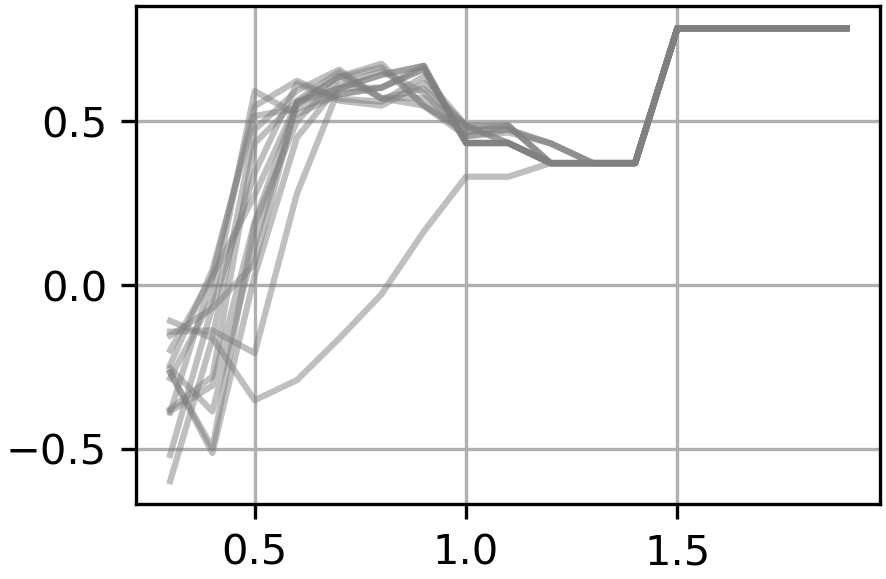
\includegraphics[width=0.4\linewidth]{pictures/Пучок кривых}
	\hspace{0.05\linewidth}
	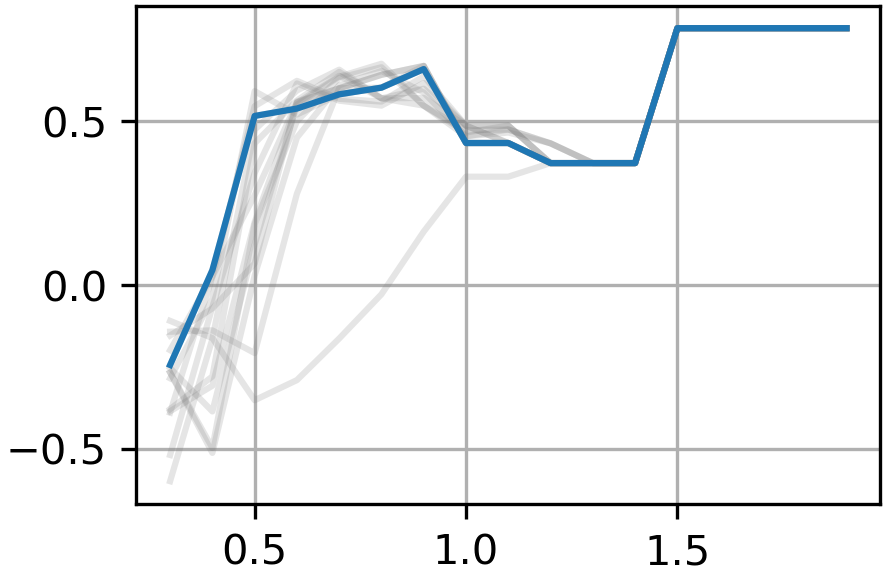
\includegraphics[width=0.4\linewidth]{pictures/Лучшая кривая}\\
	\caption{Семейство кривых и лучшая кривая}
\end{figure}

\medskip\noindent
На рисунке 3(b) изображена кривая, которая получается извлечением из таблицы \texttt{result} строки с индексом \texttt{min\_samples\_best}.


\subsection{Локтевая точка на лучшей кривой}


Мы уже отмечали что наилучшая кластеризация не всегда соответствует лучшей метрике силуэта, и что для определения оптимальных параметров кластеризации нужно использовать локтевое значение метрики (см. рис. 4(b)). 

\begin{figure}[!h]
	\centering
	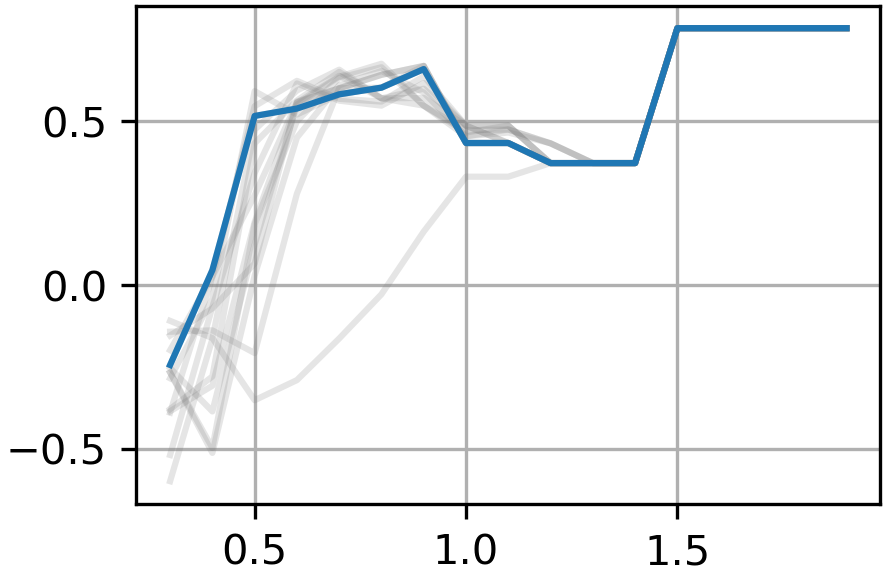
\includegraphics[width=0.4\linewidth]{pictures/Лучшая кривая}
	\hspace{0.05\linewidth}
	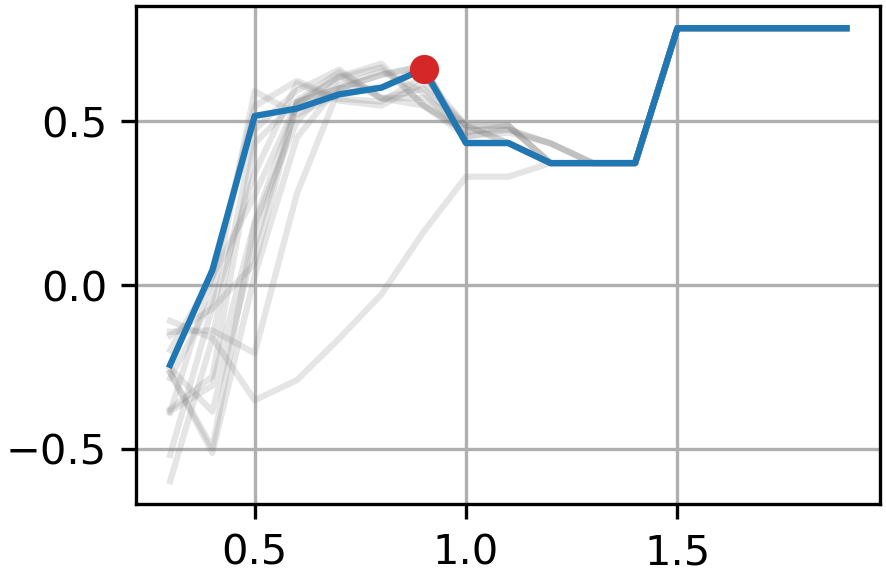
\includegraphics[width=0.4\linewidth]{pictures/Локтевая точка на лучшей кривой}\\
	\caption{Лучшая кривая и локтевая точка на лучшей кривой}
\end{figure}

На этом шаге мы применяем функцию \texttt{fold\_point}. Создаем массив предиктора:

\medskip\noindent
\texttt{A = np.array(result.columns)}

\medskip\noindent
Напомним, что в качестве горизонтальной переменной выступает параметр \texttt{eps}, то есть, массив \texttt{A} — это значения горизонтальной переменной для лучшей кривой метрики силуэта (см. рис. 4(b)). Далее, создаем массив функции, анализируемой на предмет локтевой точки:

\medskip\noindent
\texttt{B = result.iloc[min\_samples\_best].to\_numpy()}

\medskip\noindent
Массив \texttt{B} — это лучшая строка в таблице результатов, переведенная в формат массива \texttt{numpy} при помощи метода \texttt{to\_numpy}. Визуализация массивов \texttt{A} и \texttt{B} дает изображение лучшей кривой из семейства кривых метрики силуэта (см. рис. 4(b)).

После этого применяем функцию \texttt{fold\_point} к паре массивов \texttt{A} и \texttt{B}. Получаем номер предиктора, при котором наблюдается локтевое значение метрики, и записываем его в переменную \texttt{fold\_ind}:

\medskip\noindent
\texttt{fold\_ind = fold\_point(A, B)}


\subsection{Оптимальные параметры кластеризации}


Выше мы получили лучшее значение для параметра \texttt{min\_samples} и записали его в переменную \texttt{min\_sample\_best}. Теперь, пользуясь найденным номером локтевой точки, мы находим оптимальное значение параметра \texttt{eps} и записываем его в переменную \texttt{eps\_best}:

\medskip\noindent
\texttt{eps\_best = result.columns[fold\_ind]}

\subsection{Оптимальная кластеризация}


Выяснив, при каких значениях параметров \texttt{eps} и \texttt{min\_samples} кластеризация DBSCAN дает приемлемые в смысле метода локтя результаты, проводим кластеризацию исходного множества \texttt{X} с найденными значениями параметров:

\medskip\noindent
\texttt{clust = DBSCAN(eps=eps\_best, min\_samples=min\_samples\_best)\\
clust.fit(X)
}\texttt{}


\section{Результаты}

Одной из интересных особенностей кластеризации DBSCAN является то, что точки, которые с ее точки зрения не могут принадлежать никакому кластеру, выделяются в отдельный набор точек: в набор выбросов. Мы провели множественные эксперименты на синтетических данных и обнаружили, что доля выбросов в кластеризации DBSCAN связана с формой кривой метрики силуэта, соотнесенной с радиусом кластеризации (то есть, с величиной параметра \texttt{eps}). Заметим, что такой же связи с кривой метрики силуэта, соотнесенной с параметром \texttt{min\_samples}, мы не обнаружили.


\subsection{Четкое разбиение}


Если кривая метрики силуэта, соотнесенной с радиусом кластеризации, обладает ярко выраженной локтевой точкой, то, как правило, определенные нашим алгоритмом оптимальные значения параметров \texttt{eps=eps\_best} и \texttt{min\_samples=min\_samples\_best} дают четкое разбиение на кластеры с незначительной долей выбросов (см. рис. 5).

\begin{figure}[!h]
	\centering
	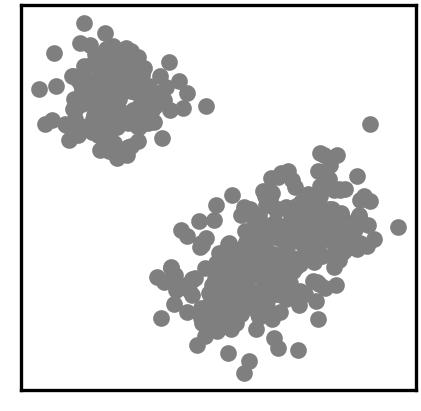
\includegraphics[width=0.25\linewidth]{pictures/Облако. Четко}
	\hspace{0.05\linewidth}
	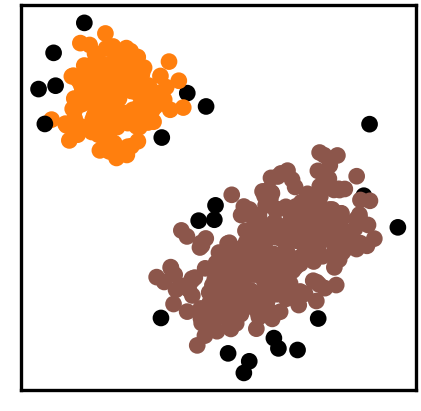
\includegraphics[width=0.25\linewidth]{pictures/Кластеры. Четко}\\
	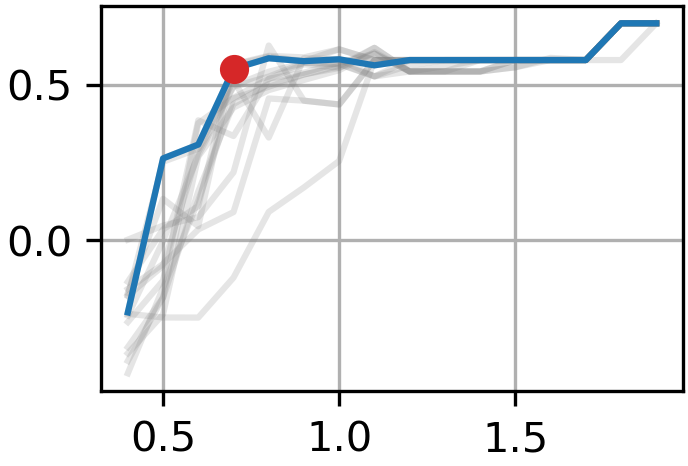
\includegraphics[width=0.42\linewidth]{pictures/Параметры. Четко}
	\\
	\caption{Четкое разбиение}
\end{figure}

Это явление наблюдается не всегда, то есть, локтевая точка может быть выраженной ярко, но, тем не менее, разбиение на кластеры будет нечетким. Однако такая ситуация встречается не часто, и в случае ярко выраженной локтевой точки характерным является именно четкое разбиение, проиллюстрированное рисунком 5.

\subsection{Разбиение с высокой долей шума}


Ели же локтевая точка на кривой метрики силуэта, соотнесенной с радиусом кластеризации, выражена неярко, то, как правило, после проведения кластеризации с найденными значениями параметров \texttt{eps=eps\_best} и\texttt{ min\_samples=min\_samples\_best} получается нечеткое разбиение с большой долей выбросов (см. рис. 6).

\begin{figure}[!h]
	\centering
	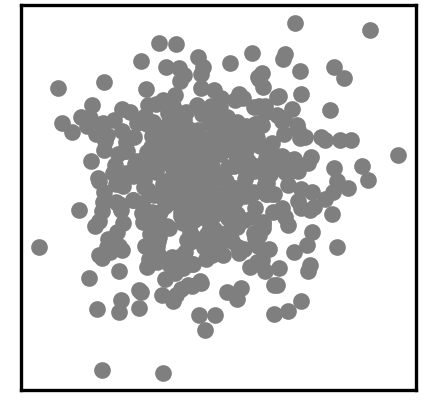
\includegraphics[width=0.25\linewidth]{pictures/Облако. Мазня}
	\hspace{0.05\linewidth}
	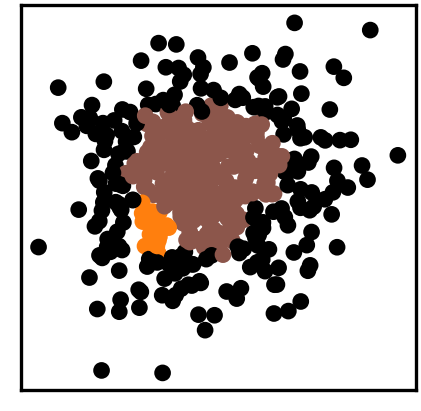
\includegraphics[width=0.25\linewidth]{pictures/Кластеры. Мазня}\\
	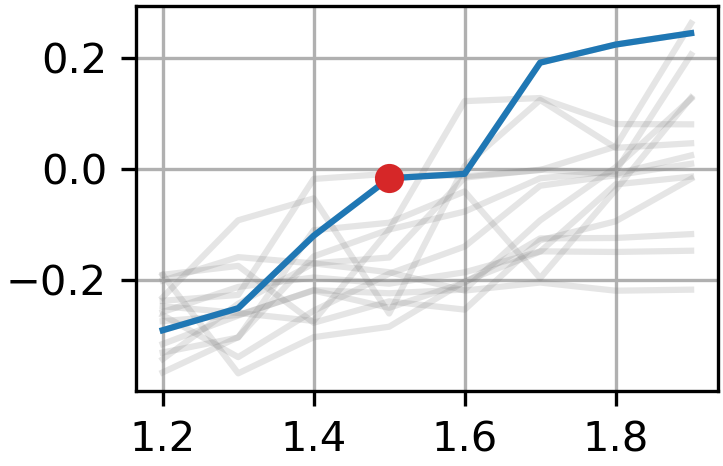
\includegraphics[width=0.42\linewidth]{pictures/Параметры. Мазня}
	\\
	\caption{Разбиение с высокой долей шума}
\end{figure}


\section{Выводы}


Итак, есть ручная настройка параметров кластеризации DBCSAN, основанная на визуальном анализе кривой метрики силуэта, и есть автоматическая настройка, основанная на модельном подходе к определению локтевой точки. 

Вне всяких сомнений, ручная настройка точнее отражает специфику данных и дает исследователю возможность выполнить кластеризацию, отталкиваясь от природы данных и особенностей задач, решаемых за счет кластеризации. Однако предложенная нами автоматическая настройка обладает как минимум двумя преимуществами:

\medskip\noindent
\begin{enumerate}
	\item она выполняется без участия аналитика, что, безусловно, играет решающую роль в ситуациях, когда кластеризация должна осуществляться многократно и/или в режиме реального времени
	\item она не допускает грубых ошибок, то есть, предлагая, возможно, не самый лучший вариант кластеризации, она никогда не предлагает неприемлемых вариантов.
\end{enumerate}

\medskip\noindent
В целом, изложенный в настоящей статье алгоритм автоматической настройки параметров кластеризации DBSCAN продемонстрировал хорошие результаты и может быть рекомендован как один из рабочих инструментов анализа данных.

\section{Литература}

\begin{enumerate}
	\item Хейдт М. Изучаем Pandas / М. Хейдт;  — Москва: ДМК Пресс, 2018. — 438 с.
	\item Бурков А. Машинное обучение без лишних слов / А. Бурков;  — СПб: Питер, 2020. — 192 с.
	\item Вьюгин, В. В. Математические основы теории машинного обучения и прогнозирования / В. В. Вьюгин; — М.: МЦИМО. — 2013. — 387~с.
	\item Бринк Х. Машинное обучение / Х. Бринк, Дж. Ричардс, М. Феверолф  — СПб.: Питер, 2017. — 336 с.
	\item В. Г. Мосин, А. В. Караваев. О некоторых проблемах моделирования измеряемых социально-психологических переменных. Математическое образование в современном мире: теория и практика : сборник статей // Самарский государственный технический университет. Всероссийская научно-методическая конференция с международным участием (28-–30 ноября 2022~г; Самара); ред. О. В. Юсупова.~--- Самара, 2022.~--- 175 с.
	\item Мосин В.Г. Линеаризация целевой функции в регрессионных задачах методом сингулярных разложений // В книге: Математическое моделирование. Тезисы II Международной конференции. Москва, 2021. С. 66--67.
\end{enumerate}




\end{document}
